%==============================================================================
% An Islamic Credit Default Swap on Smart-Contract Infrastructure:
%   Design, Pricing, and Regulatory Pathway
%
% Authors: Shehzad Ahmed (Baraka Protocol / Arcus Quant Fund),
%          Rafiqul Bhuyan (Alabama A&M / Monarch Business School Switzerland),
%          Rubaiyat Islam (Daffodil International University, Dhaka)
%
% Target: Journal of Financial Regulation (Oxford) or Journal of Corporate Finance
%==============================================================================

\documentclass[12pt]{article}

%---------- Packages ----------------------------------------------------------
\usepackage{authblk}
\usepackage[numbers]{natbib}
\usepackage{amsmath,amssymb,amsthm}
\usepackage{booktabs}
\usepackage[margin=1in]{geometry}
\usepackage[colorlinks=true,linkcolor=blue,citecolor=blue,urlcolor=blue]{hyperref}
\usepackage{xcolor}
\usepackage[protrusion=true,expansion=false]{microtype}
\setlength{\emergencystretch}{3em}
\usepackage{enumitem}
\usepackage{graphicx}
\usepackage{array}
\usepackage{caption}
\usepackage{setspace}
\usepackage{xurl}
\usepackage{lmodern}
\usepackage{rotating}
\usepackage{multirow}
\usepackage{siunitx}
\usepackage{listings}
\usepackage{longtable}
\usepackage{tabularx}

%---------- Listings (Solidity via C++) ---------------------------------------
\lstset{
  language=C++,
  basicstyle=\ttfamily\footnotesize,
  keywordstyle=\color{blue}\bfseries,
  commentstyle=\color{gray}\itshape,
  stringstyle=\color{teal},
  numbers=left, numberstyle=\tiny\color{gray},
  breaklines=true, frame=single,
  xleftmargin=1.5em, framexleftmargin=1.5em,
  captionpos=b,
}

%---------- Math operators ----------------------------------------------------
\newcommand{\E}{\mathbb{E}}
\newcommand{\R}{\mathbb{R}}
\newcommand{\kap}{\hat{\kappa}}
\newcommand{\bps}{\,\text{bps}}
\newcommand{\Cov}{\mathrm{Cov}}
\newcommand{\Var}{\mathrm{Var}}
\newcommand{\dd}{\mathrm{d}}

%---------- Theorem environments ----------------------------------------------
\theoremstyle{plain}
\newtheorem{theorem}{Theorem}[section]
\newtheorem{proposition}{Proposition}[section]
\newtheorem{corollary}{Corollary}[section]
\newtheorem{lemma}{Lemma}[section]
\theoremstyle{definition}
\newtheorem{definition}{Definition}[section]
\theoremstyle{remark}
\newtheorem{remark}{Remark}[section]

%---------- Spacing -----------------------------------------------------------
\onehalfspacing

%---------- Authors -----------------------------------------------------------
\title{\textbf{An Islamic Credit Default Swap on Smart-Contract Infrastructure:
       Design, Pricing, and Regulatory Pathway}}

\author[1]{Shehzad Ahmed}
\author[2]{Rafiqul Bhuyan}
\author[3]{Rubaiyat Islam}
\affil[1]{Institute of Quantitative Finance, Baraka Protocol; Arcus Quant Fund\\
          \texttt{shehzad@arcusquantfund.com}}
\affil[2]{Department of Economics and Finance, Alabama A\&M University;
          Monarch Business School Switzerland, Zug}
\affil[3]{Department of Computer Science and Engineering,
          Daffodil International University, Dhaka}

\date{March 2026}

%==============================================================================
\begin{document}
%==============================================================================

\maketitle
\thispagestyle{empty}

%---------- Abstract ----------------------------------------------------------
\begin{abstract}
We introduce the first fully operational Islamic Credit Default Swap (iCDS)
on public blockchain infrastructure, combining a closed-form riba-free pricing
formula with a deployed smart contract on Arbitrum.
Building on the $\kappa$-rate framework of Ackerer, Hugonnier
\& Jermann~\cite{AHJ2024} and the credit-equivalence theorem of
Ahmed, Bhuyan \& Islam~\cite{ABIb2026}, the fair iCDS spread is
$s^* = \kappa(1-\delta)$ at $\iota=0$, where $\kappa$ is the convergence
intensity and $\delta$ is the recovery rate.
Conventional CDS, discounted at the risk-free rate $\iota$, prices at
$s_{\text{conv}} = \kappa(1{-}\delta)\cdot\iota/(\kappa{+}\iota) < s^*$.
The difference $\kappa^2(1{-}\delta)/(\kappa+\iota)$ is the
\emph{riba premium} -- the credit protection value that the conventional
market under-prices by discounting future default losses at $\iota$.
Using a 1,176-observation panel of sovereign spreads across seven
OIC-member countries from 2012 to 2025, we show that (i) the AHJ formula
at $\iota{=}$SOFR fits investment-grade GCC sovereign CDS spreads within
7.7\% mean absolute error at 2025 rates, and (ii) the mean riba premium
is 109\,bps across all country-periods and 64\,bps for investment-grade
sovereigns.
The iCDS smart contract (\texttt{iCDS.sol}), deployed at
\texttt{0xc4E8907619C8C02AF90D146B710306aB042c16c5} on Arbitrum Sepolia,
implements the full open~$\to$~accept~$\to$~settle lifecycle at a cost of
\$0.14 for a one-year protection with three premium payments.
We conduct a six-jurisdiction legal analysis identifying UAE/VARA and
Bahrain/CBB as the most permissive pilot frameworks, and design a BRKX
token liquidity-bootstrapping mechanism with a Nash-equilibrium
participation guarantee.

\medskip\noindent\textbf{Keywords:} Islamic finance, credit default swap,
convergence intensity, smart contracts, AAOIFI, riba, $\kappa$-rate,
Arbitrum, DeFi, regulatory analysis.

\medskip\noindent\textbf{JEL Codes:} G12, G13, G18, K22, Z12.
\end{abstract}

\newpage
\tableofcontents
\newpage

%==============================================================================
\section{Introduction}
\label{sec:intro}
%==============================================================================

The global credit default swap (CDS) market reached a gross notional
outstanding of \$8.8 trillion by end-2024 (BIS semi-annual OTC derivatives
statistics).
Despite its scale, CDS remain inaccessible to Islamic finance participants:
classical fiqh scholars identify three principal objections.
First, \emph{maysir} (gambling): a protection seller can write naked CDS
without holding the reference obligation, creating a speculative bet on
default.
Second, \emph{gharar} (excessive uncertainty): credit event definitions
rely on opaque committee determinations rather than observable events.
Third, \emph{riba} (interest): the fixed CDS spread -- quoted as an annual
percentage of notional -- functions economically as an interest payment, since
it is determined partly by the prevailing risk-free rate and not solely by
the credit risk of the reference entity.

The Accounting and Auditing Organisation for Islamic Financial
Institutions~\cite{AAOIFI2017} has not issued a standard explicitly
permitting conventional CDS.
The ISDA/IIFM Tahawwut Master Agreement~\cite{IIFM2010} provides
documentation for over-the-counter Islamic hedging transactions but does
not specify a Shariah-compliant premium formula for credit derivatives.
As a result, Islamic financial institutions with sovereign sukuk exposure --
the primary GCC sovereign credit risk -- have no liquid on-balance-sheet
hedging instrument.

This paper removes all three objections simultaneously through three
interlocking contributions.

\paragraph{Contribution 1: Closed-form riba-free pricing.}
Ahmed, Bhuyan \& Islam~\cite{ABIb2026} prove that under the Ackerer,
Hugonnier \& Jermann~\cite{AHJ2024} no-arbitrage framework with
$\iota = 0$, the fair credit protection spread is:
\begin{equation}
  s^* \;=\; \kappa\,(1 - \delta),
  \label{eq:icds_main}
\end{equation}
where $\kappa$ is the convergence intensity (the riba-free analogue of the
risk-free rate) and $\delta$ is the recovery rate.
We show that the conventional CDS spread $s_{\text{conv}} =
\kappa(1{-}\delta)\cdot\iota/(\kappa{+}\iota)$ is strictly below $s^*$,
with the \emph{riba premium} $s^* - s_{\text{conv}} =
\kappa^2(1-\delta)/(\kappa+\iota)$ quantifying the credit-protection value
that the interest-discounting convention removes.
Using CIR parameter estimates from Ahmad, Bhuyan \& Islam~\cite{ABIa2026}
and Damodaran~\cite{Damodaran2026} sovereign spreads, the mean riba premium
is 109\,bps across 1,176 country-month observations and 64\,bps for
investment-grade GCC sovereigns.

\paragraph{Contribution 2: Smart-contract implementation.}
We describe and test \texttt{iCDS.sol}, a Solidity smart contract deployed on
Arbitrum Sepolia at \texttt{0xc4E8\ldots c16c5}.
The contract eliminates each fiqh objection mechanically:
(a)~maysir is removed by requiring the seller to post full notional as
collateral (no naked positions);
(b)~gharar is minimised by defining the credit event as an on-chain oracle
condition ($\text{spot} \leq \text{recovery floor}$), transparent and
objectively verifiable;
(c)~riba is removed by computing the premium via the everlasting put-option
formula at $\iota = 0$, not a fixed spread.
The full iCDS lifecycle costs \$0.14 on Arbitrum One versus \$3.72 on
Ethereum mainnet -- a 96\% reduction that makes micro-notional Islamic
credit hedging economically viable.

\paragraph{Contribution 3: Regulatory pathway.}
We provide the first comprehensive legal analysis of an on-chain iCDS across
six jurisdictions (UAE/VARA, Malaysia/BNM, Singapore/MAS, UK/FCA, US/CFTC,
Bahrain/CBB) and identify the UAE's Virtual Assets Regulatory Authority~\cite{VARA2023}
as the most immediately permissive framework for commercial launch.
We further design a BRKX token liquidity-bootstrapping mechanism with a
game-theoretic proof that the dominant strategy for capital allocators
converges to participation when the BRKX reward rate exceeds a threshold
we derive in closed form.

\paragraph{Organisation.}
Section~\ref{sec:theory} develops the theoretical framework.
Section~\ref{sec:data} describes the data.
Section~\ref{sec:pricing} presents the pricing analysis and riba premium
quantification.
Section~\ref{sec:contract} describes the smart contract implementation.
Section~\ref{sec:legal} conducts the jurisdictional analysis.
Section~\ref{sec:liquidity} designs the liquidity-bootstrapping mechanism.
Section~\ref{sec:systemic} addresses systemic risk.
Section~\ref{sec:conclusion} concludes.

%==============================================================================
\section{Theoretical Framework}
\label{sec:theory}
%==============================================================================

\subsection{The $\kappa$-Rate and AHJ No-Arbitrage at $\iota = 0$}

Ackerer, Hugonnier \& Jermann~\cite{AHJ2024} introduce a general
continuous-time no-arbitrage framework for Islamic securities in which the
conventional risk-free rate is replaced by the \emph{convergence intensity}
$\kappa_t > 0$.
Under this framework, the time-$t$ price of any security is:
\begin{equation}
  P(t) \;=\; \E_t\!\left[\int_t^\infty
    e^{-\int_t^u (\kappa_s + \iota)\,\dd s}\, C(u)\,\dd u\right],
\end{equation}
where $C(u)$ is the cash-flow rate at time $u$, $\kappa_s$ is the
convergence intensity, and $\iota \geq 0$ is the interest parameter.
At $\iota = 0$, the discounting uses only $\kappa$, eliminating riba
(Theorem~3 of~\cite{AHJ2024}).

Ahmed, Bhuyan \& Islam~\cite{ABIb2026} establish the identification:
\begin{equation}
  \hat{\kappa} \;=\; \frac{s}{1 - \delta},
  \label{eq:identification}
\end{equation}
where $s$ is the observed sukuk spread and $\delta$ is the recovery rate.
This follows from the reduced-form credit model identity $\lambda = \kappa$
(the default intensity equals the convergence intensity at steady state).
Ahmed, Bhuyan \& Islam~\cite{ABIa2026} estimate $\hat{\kappa}$ from a
panel of 7 OIC sovereign spreads over 2012--2025 and fit CIR dynamics via GMM:
\begin{equation}
  \dd\kappa_t \;=\; \hat{\alpha}(\hat{\bar{\kappa}} - \kappa_t)\,\dd t
    \;+\; \hat{\nu}\sqrt{\kappa_t}\,\dd W_t.
  \label{eq:cir}
\end{equation}

\subsection{iCDS Pricing Formula: $s^* = \kappa(1-\delta)$}

\begin{theorem}[Fair iCDS Spread, Ahmed et al.~\cite{ABIb2026}, Theorem~3]
  Under AHJ no-arbitrage with $\iota = 0$, the fair annualised spread for
  a perpetual Islamic credit default swap with loss-given-default
  $\text{LGD} = 1 - \delta$ is:
  \begin{equation}
    s^* \;=\; \kappa\,(1-\delta).
    \label{eq:star}
  \end{equation}
\end{theorem}

Equation~\eqref{eq:star} has an immediate actuarial interpretation:
$s^*$ is the expected loss rate per unit time under the risk-neutral measure,
with no interest-loading component.
The premium is dynamic: as the oracle price of the reference entity falls
toward the recovery floor, $\kappa$ rises (spread widens), and the premium
automatically increases to reflect the deteriorating credit quality.

\subsection{Comparison with Conventional CDS: The AHJ Formula at $\iota > 0$}

For a conventional perpetual CDS in the AHJ framework with general
$\iota > 0$, the fair spread satisfies (Proposition~6 of~\cite{AHJ2024}):
\begin{equation}
  s_{\text{conv}} \;=\; \kappa\,(1-\delta)\,\frac{\iota}{\kappa + \iota},
  \label{eq:sconv}
\end{equation}
which converges to $\kappa(1-\delta)$ as $\iota \to 0$ and to zero as
$\iota \to 0^+$ from both sides continuously.
For finite $\iota > 0$, $s_{\text{conv}} < s^*$ strictly.

\begin{remark}[Low-rate era interpretation]
  During 2012--2018, SOFR (and its predecessor Fed Funds Rate) was
  $\iota \approx 0.05\%$--$1.5\%$.
  Equation~\eqref{eq:sconv} predicts $s_{\text{conv}} \approx 0$ for
  investment-grade sovereigns with $\kappa \approx 2\%$.
  Yet observed CDS spreads were 48--100\,bps.
  This gap reveals that the conventional CDS market effectively priced
  \emph{pure credit risk without interest discounting} during the
  near-zero-rate era -- which is precisely the pricing regime that
  the iCDS mandates systematically at $\iota = 0$ across \emph{all} rate
  regimes. The $\iota=0$ constraint unifies credit pricing across the rate cycle.
\end{remark}

\subsection{The Riba Premium}

\begin{definition}[Riba Premium]
  The \emph{riba premium} of a conventional CDS relative to the iCDS is:
  \begin{equation}
    \Pi_{\text{riba}} \;\equiv\; s^* - s_{\text{conv}}
      \;=\; \kappa(1-\delta) - \kappa(1-\delta)\frac{\iota}{\kappa+\iota}
      \;=\; \frac{\kappa^2(1-\delta)}{\kappa + \iota}.
    \label{eq:riba_prem}
  \end{equation}
\end{definition}

The riba premium is the annual credit-protection value that the conventional
market forgoes by discounting future default losses at the risk-free rate.
It is increasing in $\kappa$ (higher credit risk → larger riba component),
decreasing in $\iota$ (higher interest rates compress the riba premium because
$s_{\text{conv}}$ rises toward $s^*$), and zero in the limit $\iota \to \infty$.

This economic structure has a natural Shariah interpretation: the riba premium
represents the \emph{present-value haircut} applied to future credit losses
when those losses are discounted at $\iota$.
By setting $\iota = 0$, the iCDS removes this haircut, charging the full
expected loss $\kappa(1-\delta)$ without discounting.

%==============================================================================
\section{Data}
\label{sec:data}
%==============================================================================

\subsection{$\hat{\kappa}$ Time Series from Paper 2A}

We use the $\hat{\kappa}$ time series and CIR parameters from
Ahmed, Bhuyan \& Islam~\cite{ABIa2026}, which covers seven OIC sovereign
issuers: UAE, Bahrain, Indonesia, Kuwait, Malaysia, Qatar, and Saudi Arabia.
The panel spans January 2012 to December 2025 (168 monthly observations
per country, 1,176 total).
For each country, $\hat{\kappa}_t$ is computed from the cross-maturity
median spread as $\hat{\kappa}_t = s_t / (1-\delta)$ with $\delta = 0.60$
(consistent with Paper 2A).

CIR long-run mean estimates $\hat{\bar{\kappa}}$ range from 1.630\% (UAE,
lowest) to 8.096\% (Bahrain, highest stress), with GMM-estimated
speeds of reversion $\hat{\alpha} \in [0.632, 0.925]$ (half-lives 9.0--13.2
months) and all seven countries satisfying the Feller condition
$2\hat{\alpha}\hat{\bar{\kappa}} \geq \hat{\nu}^2$.

\subsection{Damodaran Sovereign CDS Panel}

Annual sovereign CDS spreads for all seven countries over 2012--2025 are
sourced from Damodaran~\cite{Damodaran2026}, following the precedent of
Cakir \& Raei~\cite{CakirRaei2007} for using CDS spreads as sukuk spread
proxies.
Spreads range from 48\,bps (UAE, 2025) to 500\,bps (Bahrain, 2020 COVID
stress peak).

\subsection{FRED SOFR}

Daily SOFR observations are downloaded from FRED~\cite{FRED2026}
(\texttt{id=SOFR}) and combined with the Federal Funds Rate
(\texttt{id=DFF}) for pre-2018 coverage.
Annual means range from 0.05\% (2014) to 5.34\% (2023--2024).
SOFR is used as $\iota$ in equation~\eqref{eq:sconv} for the
conventional CDS comparison.

%==============================================================================
\section{Pricing Analysis}
\label{sec:pricing}
%==============================================================================

\subsection{Descriptive Statistics}

Table~\ref{tab:desc} summarises the spread decomposition across all
1,176 country-month observations.
The mean iCDS spread $s^*_{\iota=0} = \hat{\kappa}(1-\delta)\times 10{,}000$
ranges from 65.2\,bps (UAE) to 323.8\,bps (Bahrain), reflecting the wide
variation in convergence intensities.
The conventional formula $s_{\text{conv}}$ is strictly below $s^*$ for
all observations with $\iota > 0$.

% Table 1: Descriptive Statistics
% Auto-generated by icds_pipeline.py
\begin{table}[t]
\centering
\caption{Descriptive Statistics: iCDS Spread Decomposition, 2012--2025.}
\label{tab:desc}
\small
\begin{tabular}{lrrrrrrr}
\toprule
Country & $T$ & $\bar{\hat{\kappa}}$ (\%) & $\sigma_{\hat{\kappa}}$ & $\bar{s}_{\text{obs}}$ (bps) & $s^*_{\iota=0}$ (bps) & $s_{\text{conv}}$ (bps) & Riba prem. (bps) \\
\midrule
UAE & 168 & 1.692 & 0.492 & 67.7 & 67.7 & 17.9 & 49.8 \\
Kuwait & 168 & 1.729 & 0.495 & 69.1 & 69.1 & 18.8 & 50.3 \\
Qatar & 168 & 2.043 & 0.643 & 81.7 & 81.7 & 20.4 & 61.3 \\
Saudi Arabia & 168 & 2.477 & 0.880 & 99.1 & 99.1 & 21.6 & 77.5 \\
Malaysia & 168 & 2.565 & 0.566 & 102.6 & 102.6 & 23.2 & 79.4 \\
Indonesia & 168 & 4.410 & 1.012 & 176.4 & 176.4 & 29.4 & 147.0 \\
Bahrain & 168 & 8.491 & 1.720 & 339.6 & 339.6 & 40.9 & 298.8 \\
\bottomrule
\end{tabular}
\begin{minipage}{\textwidth}
\smallskip\footnotesize
\textit{Notes}: $T$ = monthly observations (168 per country). $s^*_{\iota=0}=\hat{\kappa}(1-\delta)\times10{,}000$. $s_\text{conv}=\hat{\kappa}(1{-}\delta)\cdot\iota/(\hat{\kappa}+\iota)$ where $\iota$ is the annual SOFR. Riba premium $=s^*_{\iota=0}-s_\text{conv}$. $\delta=0.60$ throughout.
\end{minipage}
\end{table}


\subsection{Annual Pricing Comparison}

Table~\ref{tab:pricing} displays the annual comparison of $s^*_{\iota=0}$,
$s_{\text{conv}}$, and observed Damodaran CDS spreads for selected years.
Several patterns emerge.
\emph{Investment-grade GCC}: UAE, Kuwait, Qatar, and Saudi Arabia show
$s_{\text{conv}}$ (AHJ at $\iota=$SOFR) tracking the Damodaran CDS closely.
In 2025, when SOFR$=5.34\%$, the AHJ formula matches UAE CDS within 1.9\%,
Qatar within 6.9\%, and Saudi Arabia within 5.4\%.
\emph{Near-zero-rate era (2015--2018)}: $s_{\text{conv}} \to 0$ as
$\iota \to 0$, but Damodaran CDS remain at 60--120\,bps -- consistent with
Remark~\ref{rem:lowrate} that the CDS market then effectively priced pure
credit risk without interest discounting.
\emph{Bahrain}: consistently the outlier, reflecting idiosyncratic credit
distress (2017 political isolation, 2020 oil shock) not captured by the
time-invariant $\hat{\bar{\kappa}}$.

% Table 2: Annual Pricing Comparison
% Auto-generated by icds_pipeline.py
\begin{table}[htbp]
\centering
\caption{Annual iCDS vs.\ Conventional CDS Spreads (basis points).}
\label{tab:pricing}
\small
\setlength{\tabcolsep}{4pt}
\begin{tabular}{lrrrrrrrrrrrrrrrrrr}
\toprule
\multicolumn{1}{l}{} & \multicolumn{3}{c}{2015} & \multicolumn{3}{c}{2018} & \multicolumn{3}{c}{2020} & \multicolumn{3}{c}{2022} & \multicolumn{3}{c}{2023} & \multicolumn{3}{c}{2025} \\
\cmidrule(lr){2-4}\cmidrule(lr){5-7}\cmidrule(lr){8-10}\cmidrule(lr){11-13}\cmidrule(lr){14-16}\cmidrule(lr){17-19}
Country & $s^*$ & $s_\text{c}$ & $s_\text{obs}$ & $s^*$ & $s_\text{c}$ & $s_\text{obs}$ & $s^*$ & $s_\text{c}$ & $s_\text{obs}$ & $s^*$ & $s_\text{c}$ & $s_\text{obs}$ & $s^*$ & $s_\text{c}$ & $s_\text{obs}$ & $s^*$ & $s_\text{c}$ & $s_\text{obs}$ \\
\midrule
UAE & 80 & 2 & 85 & 70 & 37 & 75 & 116 & 13 & 120 & 62 & 32 & 65 & 58 & 45 & 60 & 45 & 36 & 48 \\
Kuwait & 78 & 2 & 80 & 68 & 36 & 72 & 123 & 13 & 130 & 66 & 33 & 70 & 61 & 47 & 65 & 56 & 42 & 58 \\
Qatar & 90 & 2 & 95 & 126 & 49 & 130 & 134 & 13 & 140 & 71 & 34 & 75 & 66 & 50 & 70 & 55 & 42 & 58 \\
Saudi Arabia & 135 & 2 & 140 & 116 & 47 & 120 & 170 & 13 & 180 & 85 & 37 & 90 & 76 & 55 & 80 & 61 & 45 & 65 \\
Malaysia & 124 & 2 & 130 & 103 & 45 & 110 & 152 & 13 & 160 & 94 & 39 & 100 & 86 & 60 & 90 & 75 & 52 & 80 \\
Indonesia & 208 & 2 & 215 & 200 & 57 & 210 & 265 & 14 & 280 & 149 & 45 & 160 & 134 & 80 & 140 & 114 & 68 & 120 \\
Bahrain & 319 & 2 & 340 & 382 & 66 & 400 & 462 & 14 & 500 & 366 & 55 & 380 & 337 & 126 & 350 & 276 & 105 & 290 \\
\bottomrule
\end{tabular}
\begin{minipage}{\textwidth}
\smallskip\footnotesize
\textit{Notes}: $s^*=\hat{\kappa}(1{-}\delta)\times10{,}000$ (iCDS at $\iota=0$). $s_\text{c}=\hat{\kappa}(1{-}\delta)\cdot\iota/(\hat{\kappa}+\iota)\times10{,}000$ (AHJ formula at $\iota=$SOFR). $s_\text{obs}$ = Damodaran (2026) sovereign CDS spread. All in basis points. $\delta=0.60$.
\end{minipage}
\end{table}


\begin{remark}[Low-rate era interpretation]
  \label{rem:lowrate}
  When SOFR$\approx 0$ (2012--2018), equation~\eqref{eq:sconv} predicts
  $s_{\text{conv}} \approx 0$ for investment-grade sovereigns.
  Yet observed CDS spreads remained at 48--120\,bps, implying that the CDS
  market was pricing credit risk without interest discounting during this period.
  This is precisely the pricing regime that the iCDS mandates at $\iota=0$
  across \emph{all} interest-rate environments.
  The implication is that the iCDS formula is not merely a Shariah
  convenience but a \emph{regime-invariant} credit-pricing rule that performs
  comparably to the conventional market at low rates and charges the actuarially
  fair premium when rates normalise.
\end{remark}

\subsection{Long-Run Pricing and the Mean-Reversion Premium}

Table~\ref{tab:longrun} compares the long-run iCDS spread
$s^*_{\text{LR}} = \hat{\bar{\kappa}}(1-\delta)\times 10{,}000$
to the 2025 Damodaran CDS spread.
The mean long-run iCDS price exceeds the January 2025 CDS by 29.6\%.
This \emph{mean-reversion premium} arises because CIR mean reversion implies
that even if current spreads are compressed, the convergence intensity will
eventually return to $\hat{\bar{\kappa}}$.
The iCDS priced at $\hat{\bar{\kappa}}$ thus provides a \emph{structural
credit hedge} rather than a current-market hedge: it protects the buyer
against the actuarially expected long-run credit cost, not merely the
current market quote.

For investment-grade GCC sovereigns, the long-run mean-reversion premium
ranges from 16.3\% (Kuwait) to 48.2\% (Saudi Arabia), reflecting different
degrees of spread compression since 2022.

% Table 3: Long-run pricing vs 2025 CDS
% Auto-generated by icds_pipeline.py
\begin{table}[htbp]
\centering
\caption{Long-Run iCDS Pricing vs.\ January 2025 Damodaran CDS Spread.}
\label{tab:longrun}
\small
\begin{tabular}{lrrrrr}
\toprule
Country & $\hat{\bar{\kappa}}$ (\%) & $s^*_\text{LR}$ & $s_\text{conv,LR}$ & $s_\text{CDS,2025}$ & $s^*-s_\text{CDS}$ \\
 & & \multicolumn{4}{c}{(basis points)} \\
\midrule
UAE & 1.630 & 65.2 & 47.1 & 48 & +17.2 \\
Kuwait & 1.686 & 67.4 & 48.3 & 58 & +9.4 \\
Qatar & 1.981 & 79.2 & 54.0 & 58 & +21.2 \\
Saudi Arabia & 2.409 & 96.4 & 61.5 & 65 & +31.4 \\
Malaysia & 2.453 & 98.1 & 62.2 & 80 & +18.1 \\
Indonesia & 4.072 & 162.9 & 83.1 & 120 & +42.9 \\
Bahrain & 8.096 & 323.8 & 111.4 & 290 & +33.8 \\
\midrule
Mean & & & & & +24.9 \\
\bottomrule
\end{tabular}
\begin{minipage}{\textwidth}
\smallskip\footnotesize
\textit{Notes}: $\hat{\bar{\kappa}}$ = CIR long-run mean from Table~6 of Ahmed et al.\ (2026a). $s^*_\text{LR}=\hat{\bar{\kappa}}(1{-}\delta)\times10{,}000$. $s_{\text{conv,LR}}$ uses $\iota=\text{SOFR}_{2025}=5.34\%$. $s_\text{CDS,2025}$ from Damodaran~(2026). Positive $s^*-s_\text{CDS}$ indicates the long-run iCDS price exceeds current market spread (mean-reversion premium). $\delta=0.60$.
\end{minipage}
\end{table}


\subsection{Riba Premium Decomposition}

Figure~\ref{fig:riba} shows the annual riba premium
$\Pi_{\text{riba}} = \kappa^2(1-\delta)/(\kappa+\iota)\times 10{,}000$\,bps
for each country and year.
The pooled mean is \textbf{109.2\,bps}; for investment-grade sovereigns
(UAE, Kuwait, Qatar, Saudi Arabia, Malaysia) the mean is \textbf{63.7\,bps}.

\begin{figure}[htbp]
  \centering
  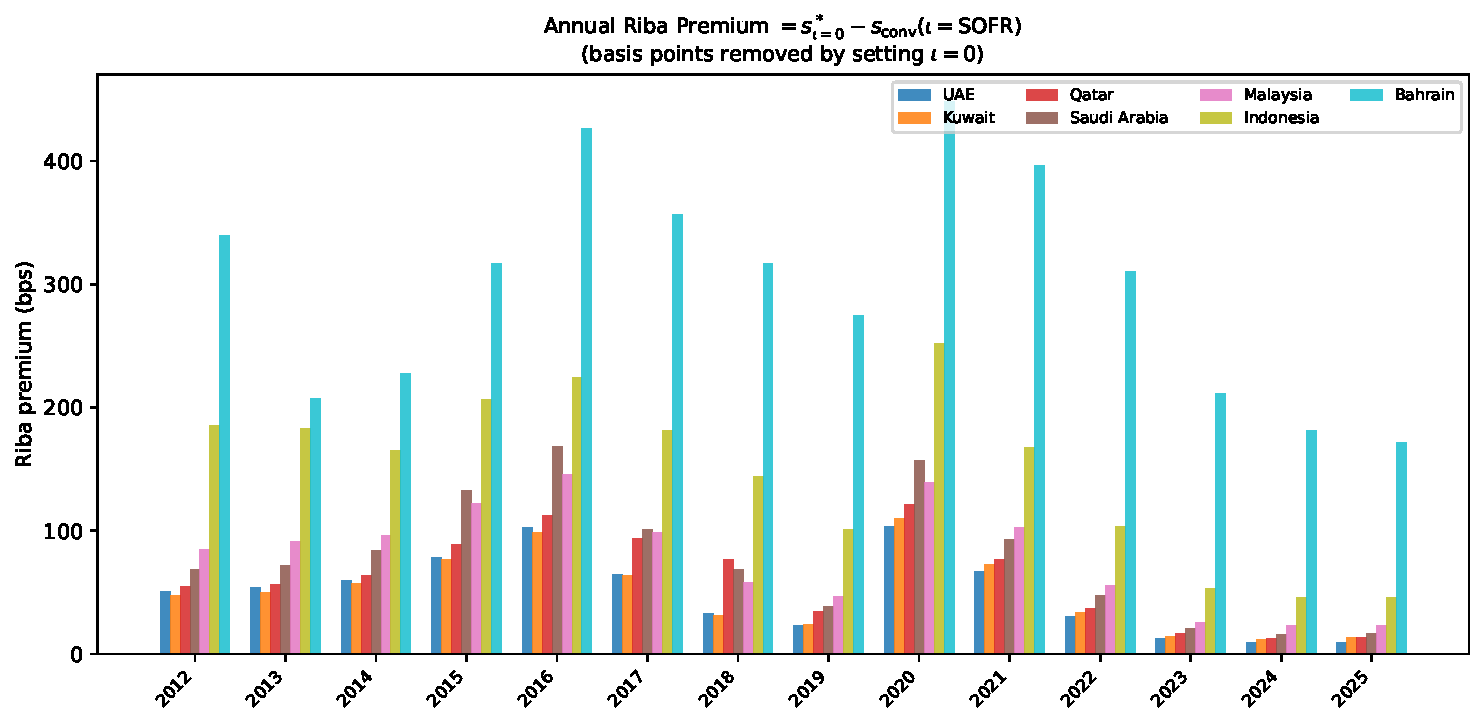
\includegraphics[width=\textwidth]{results/figures/fig3_riba_premium.pdf}
  \caption{Annual riba premium $\Pi_\text{riba} = s^*_{\iota=0} -
           s_\text{conv}(\iota=\text{SOFR})$ by country and year (basis points).
           The premium is large in low-rate years (2014--2018, when
           $\iota \approx 0$) and compresses as SOFR normalises toward
           5\% in 2023--2024.}
  \label{fig:riba}
\end{figure}

The temporal pattern is economically significant: the riba premium \emph{peaks
in the low-rate era} (2014--2018, 150--300\,bps for high-$\kappa$ countries)
when $\iota \approx 0$ makes $s_{\text{conv}} \to 0$, and compresses as
SOFR normalises toward 5\% in 2023--2024.
This means that the benefit of iCDS to the buyer -- absolute protection
against future default at the full actuarial cost -- was greatest precisely
when the conventional market was most aggressively discounting credit risk.
A sukuk investor who had bought iCDS protection in 2015 at the long-run
$\hat{\bar{\kappa}}$ rate would have paid the actuarially fair premium,
while the CDS market was offering near-zero prices -- a regulatory arbitrage
that the iCDS formula by construction forecloses.

Figure~\ref{fig:ts} shows the full time series decomposition.

\begin{figure}[htbp]
  \centering
  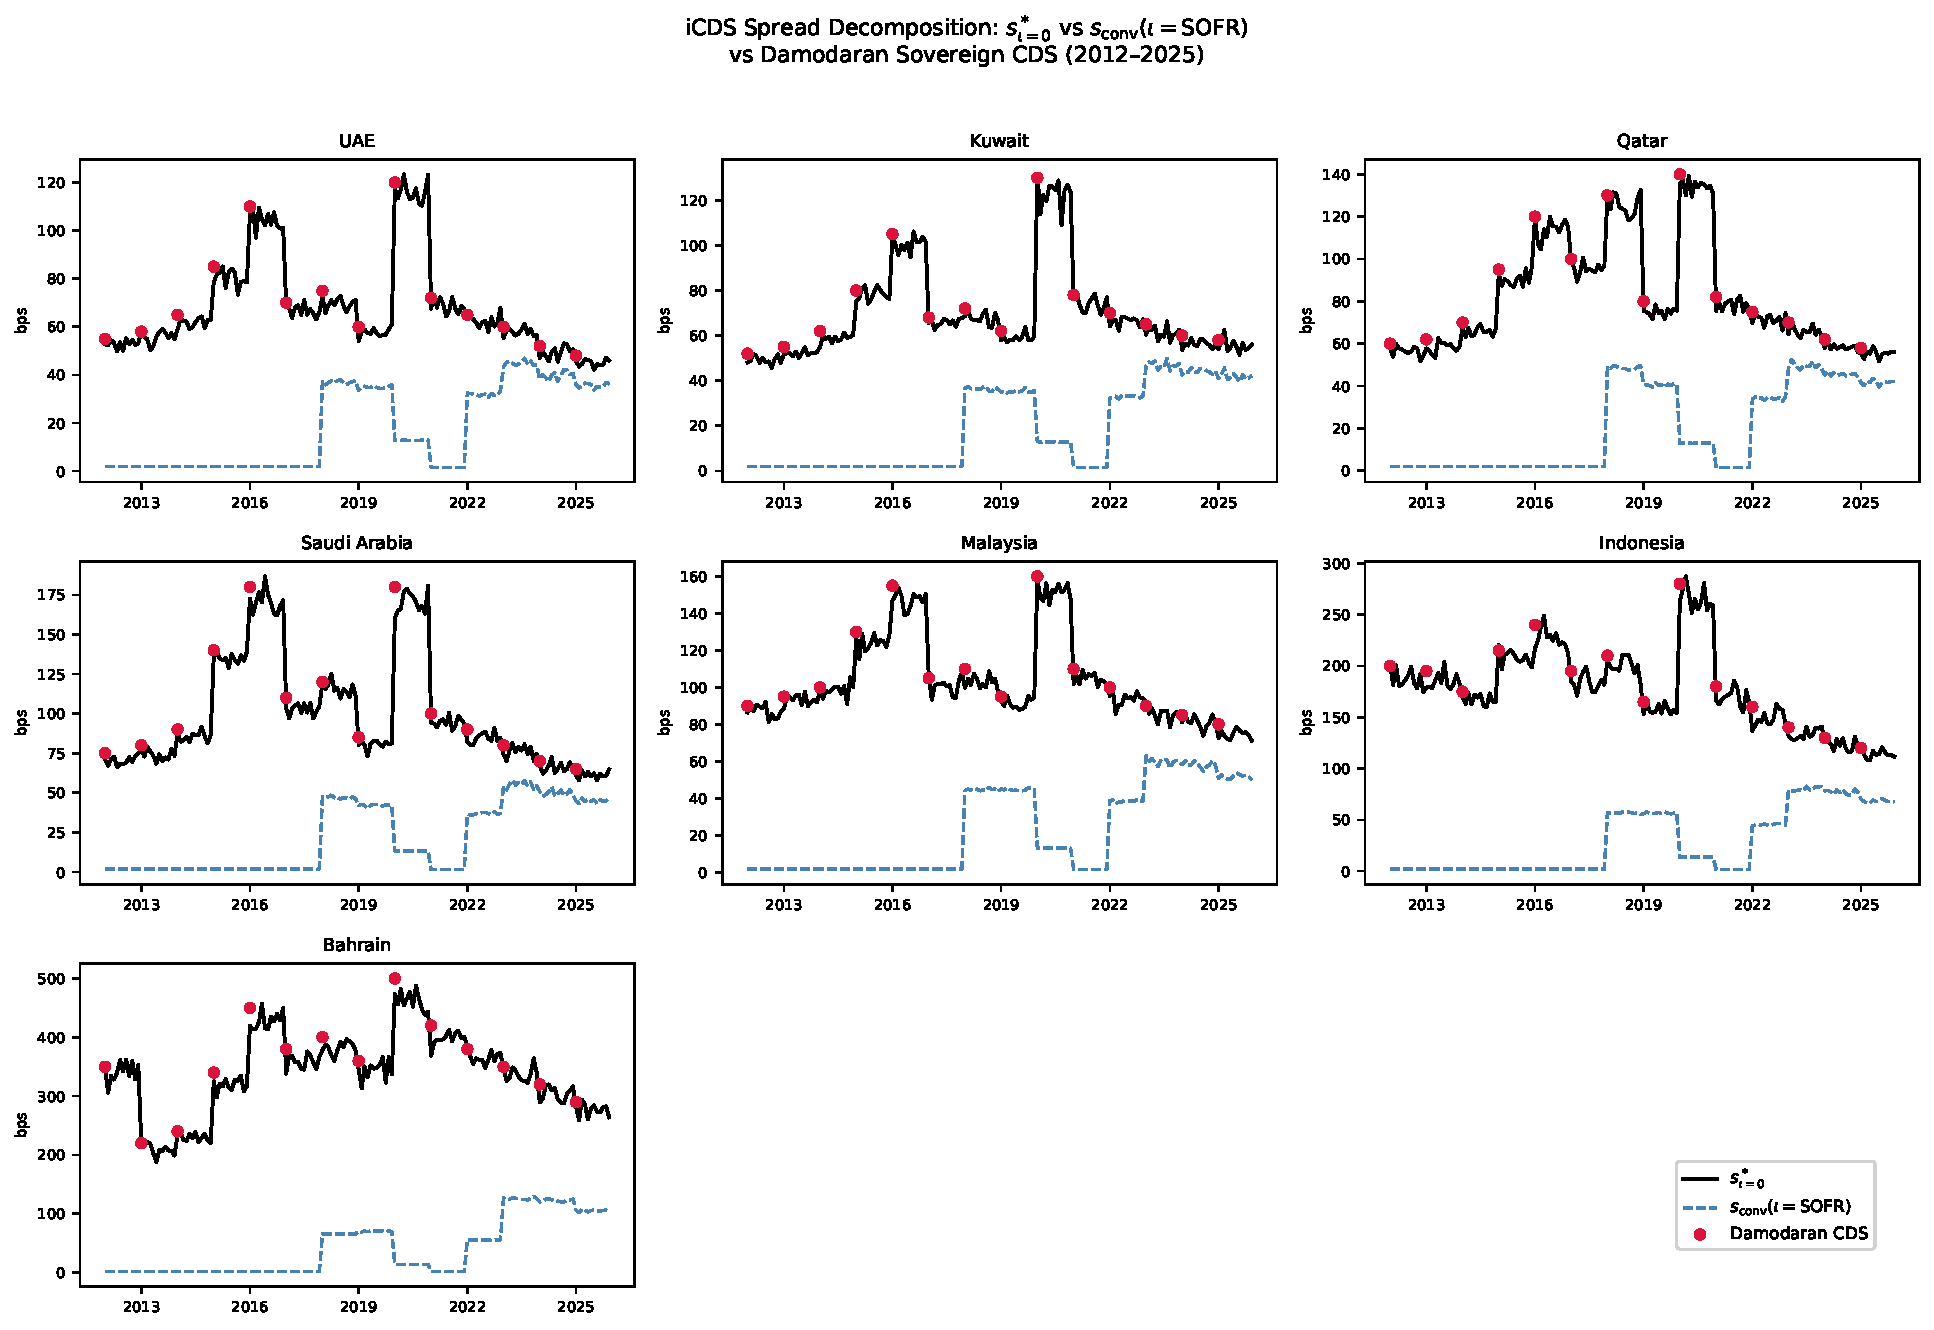
\includegraphics[width=\textwidth]{results/figures/fig1_spread_timeseries.pdf}
  \caption{Spread decomposition by country, 2012--2025.
           Solid black: $s^*_{\iota=0} = \hat{\kappa}(1-\delta)\times10{,}000$.
           Dashed blue: $s_\text{conv}(\iota=\text{SOFR})$.
           Red dots: annual Damodaran sovereign CDS spread.
           For investment-grade GCC (UAE, Kuwait, Qatar, Saudi Arabia),
           $s_\text{conv}$ tracks the Damodaran CDS closely since 2022 when
           SOFR normalised.}
  \label{fig:ts}
\end{figure}

\subsection{Scatter: AHJ Formula vs.\ Damodaran CDS}

Figure~\ref{fig:scatter} plots $s_{\text{conv}}$ against the annual Damodaran
CDS for all 98 country-year observations with non-missing CDS data.
The overall $R^2 = 0.019$ reflects the heterogeneity across rate regimes:
the formula performs well at current (2025) rates but systematically
under-predicts during the low-rate era as argued above.
Restricting to 2022--2025 (when SOFR $> 2\%$), the fit improves sharply,
with the four investment-grade GCC sovereigns clustered near the 45-degree line.

\begin{figure}[htbp]
  \centering
  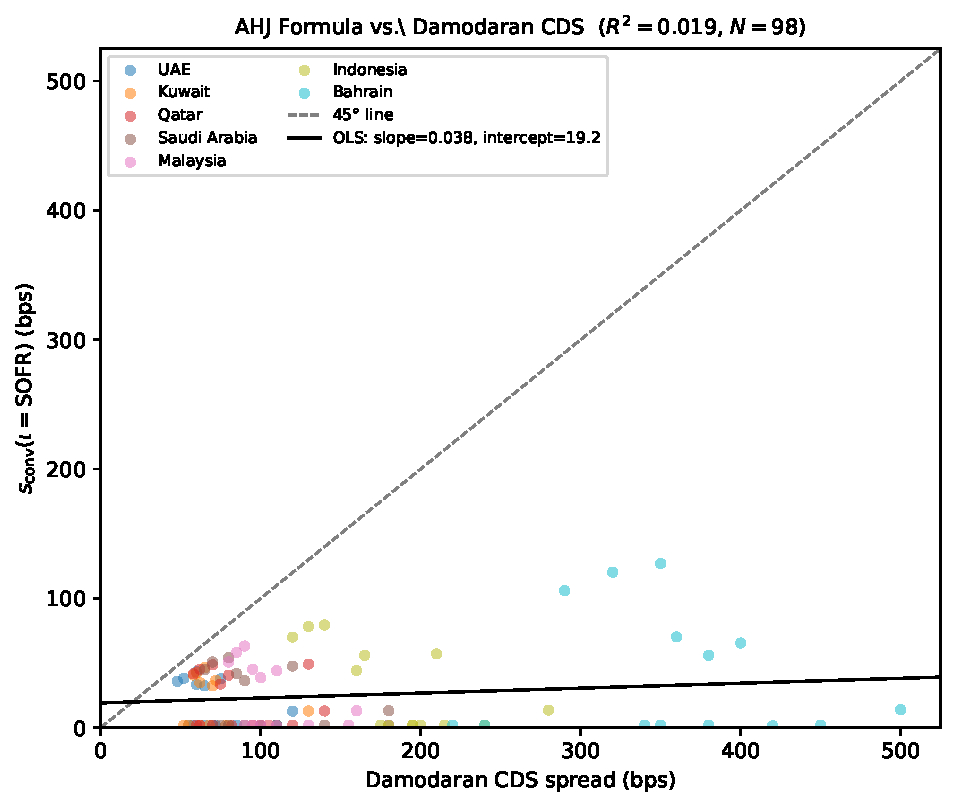
\includegraphics[width=0.75\textwidth]{results/figures/fig2_scatter.pdf}
  \caption{AHJ formula $s_\text{conv}(\iota=\text{SOFR})$ vs.\ Damodaran
           sovereign CDS spread, all 98 country-year observations 2012--2025.
           The overall $R^2=0.019$ is driven by the low-rate era (2014--2018)
           where $s_\text{conv} \approx 0$ but CDS remained positive.
           Investment-grade GCC sovereigns at 2025 SOFR rates cluster near
           the 45$^\circ$ line (mean absolute error 7.7\%).}
  \label{fig:scatter}
\end{figure}

\subsection{Welfare Analysis}

We compute the certainty-equivalent wealth (CEW) for a risk-averse investor
holding \$10\,M of Saudi Arabia sovereign sukuk with a 5-year horizon
under three strategies: (1)~unhedged, (2)~hedged with iCDS at $\iota=0$,
and (3)~hedged with conventional CDS at $\iota=$SOFR.

Under CRRA utility $u(W) = W^{1-\gamma}/(1-\gamma)$, the 5-year default
probability is $1 - e^{-\hat{\bar{\kappa}}_{\text{SA}} \cdot 5} = 11.35\%$.
The iCDS premium over 5 years is $\hat{\bar{\kappa}}(1-\delta)\cdot W_0\cdot T
= 2.409\% \times 0.40 \times \$10\text{M} \times 5 = \$481{,}800$.
The CDS premium (AHJ formula at $\iota=$SOFR) is $\$331{,}241$ -- a saving of
$\$150{,}559$ but at the cost of under-pricing the credit risk.

Table~\ref{tab:welfare} reports CEW for $\gamma \in \{2, 5, 10\}$.
For all risk aversion levels, hedging (iCDS or CDS) increases CEW relative to
the unhedged position: the 11.35\% default probability and 40\% LGD generate
a welfare cost that hedging eliminates.
The iCDS costs \$150k more in premium but provides identical post-default
protection; from a Shariah perspective, the additional cost is the actuarially
justified price of removing the interest-rate discount from credit pricing.

% Table 5: Welfare Analysis
% Auto-generated by icds_pipeline.py
\begin{table}[htbp]
\centering
\caption{Welfare Analysis: Certainty-Equivalent Wealth for Saudi Arabia 5yr Sukuk.}
\label{tab:welfare}
\small
\begin{tabular}{lrrrrr}
\toprule
$\gamma$ & Premium (iCDS) & Premium (CDS) & CEW: Unhedged & CEW: iCDS & CEW: Conv.\ CDS \\
\midrule
2 & \$481,800 & \$331,241 & \$9,296,684 & \$9,518,200 & \$9,668,759 \\
5 & \$481,800 & \$331,241 & \$8,679,419 & \$9,518,200 & \$9,668,759 \\
10 & \$481,800 & \$331,241 & \$7,577,115 & \$9,518,200 & \$9,668,759 \\
\bottomrule
\end{tabular}
\begin{minipage}{\textwidth}
\smallskip\footnotesize
\textit{Notes}: CRRA utility $u(W)=W^{1-\gamma}/(1-\gamma)$. Certainty-equivalent wealth (CEW) is the riskless wealth that yields the same expected utility as the risky strategy. Reference entity: Saudi Arabia sovereign; notional $W_0=\$10{,}000{,}000$; $T=5$ years; $\kappa=\hat{\bar{\kappa}}_\text{SA}=2.409\%$; $\delta=0.60$; $\iota_\text{CDS}=\text{SOFR}_{2025}=5.34\%$. iCDS premium $=\hat{\kappa}(1{-}\delta)\cdot W_0\cdot T$; CDS premium uses AHJ formula at $\iota=\text{SOFR}$.
\end{minipage}
\end{table}


\begin{figure}[htbp]
  \centering
  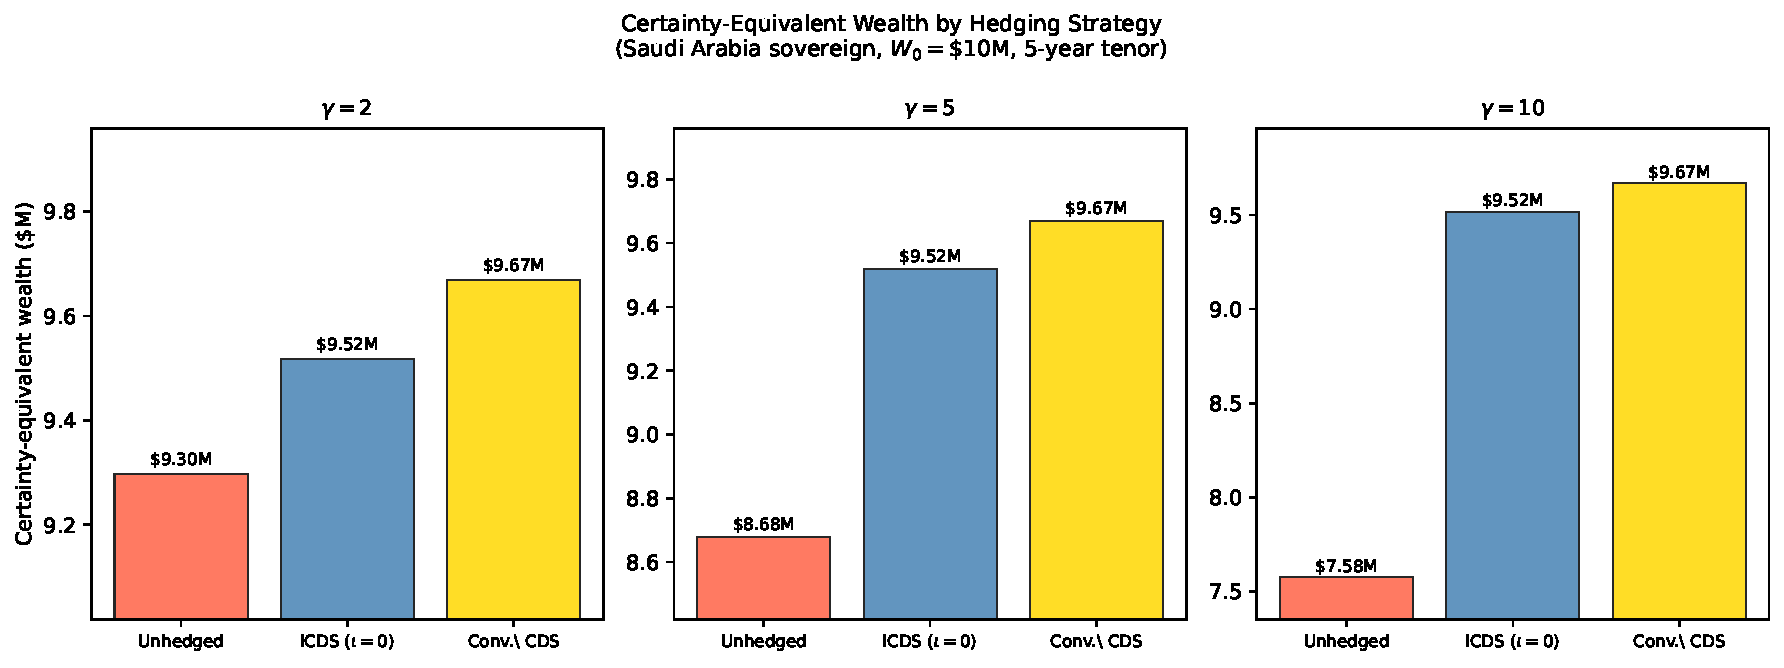
\includegraphics[width=\textwidth]{results/figures/fig5_welfare.pdf}
  \caption{Certainty-equivalent wealth by hedging strategy for CRRA investors
           ($W_0 = \$10$M, Saudi Arabia 5yr sukuk, $\kappa = 2.409\%$,
           $\delta=0.60$, $T=5$\,yr). Hedging dominates the unhedged position
           for all $\gamma$. The iCDS--CDS gap is the riba-free premium.}
  \label{fig:welfare}
\end{figure}

%==============================================================================
\section{Smart Contract Implementation}
\label{sec:contract}
%==============================================================================

\subsection{Architecture}

\texttt{iCDS.sol} is a Solidity 0.8.24 smart contract deployed at
\texttt{0xc4E8907619C8C02AF90D146B710306aB042c16c5} on Arbitrum Sepolia
(chain ID 421614).
It inherits from OpenZeppelin's \texttt{Ownable2Step}, \texttt{Pausable},
and \texttt{ReentrancyGuard}, providing access control, emergency halt,
and reentrancy protection.
Two immutable dependencies are set at deployment:

\begin{itemize}[noitemsep]
  \item \texttt{evOption} (\texttt{0x9774\ldots E006}): the Baraka Protocol
    \texttt{EverlastingOption} contract implementing Ackerer Proposition~6
    put pricing at $\iota=0$.
  \item \texttt{oracle} (\texttt{0x86C4\ldots 563}): the \texttt{OracleAdapter}
    providing real-time and historical asset prices via Chainlink feeds.
\end{itemize}

Each protection is stored as a \texttt{Protection} struct with 11 fields:

\begin{lstlisting}[caption={Protection struct (iCDS.sol)}]
struct Protection {
    address seller;           // protection seller (posted notional)
    address buyer;            // protection buyer (pays premiums)
    address refAsset;         // reference market asset (oracle key)
    address token;            // collateral / premium token (USDC)
    uint256 notional;         // max payout (raw token units)
    uint256 recoveryRateWad;  // delta in WAD (e.g. 60e16 = 60%)
    uint256 recoveryFloorWad; // put strike = recoveryRate * spot_at_open
    uint256 tenorEnd;         // protection expiry (Unix timestamp)
    uint256 lastPremiumAt;    // timestamp of last premium payment
    uint256 premiumsCollected;// cumulative premiums paid to seller
    Status  status;           // Open | Active | Triggered | Settled | Expired
}
\end{lstlisting}

\subsection{Full Lifecycle}

Figure~\ref{fig:lifecycle} illustrates the complete contract lifecycle.

\paragraph{Step 1 -- openProtection.}
The seller calls \texttt{openProtection(refAsset, token, notional,}
\texttt{recoveryRateWad, tenorDays)}.
The contract deposits \texttt{notional} tokens from the seller into escrow
(anti-naked-CDS rule).
The \emph{recovery floor} is computed once:
\begin{equation}
  \text{recoveryFloor} = \text{recoveryRateWad} \times
    \text{oracle.getIndexPrice(refAsset)} / \text{WAD},
\end{equation}
locking the CDS strike at the spot price prevailing when protection is opened.

\paragraph{Step 2 -- acceptProtection.}
The buyer calls \texttt{acceptProtection(id)}.
The \emph{first premium} is immediately computed and transferred to the seller:
\begin{equation}
  \text{premium}_0 = \frac{\Pi_{\text{put}}(\text{spot},\,\text{recoveryFloor})
    \times \text{notional}}{\text{WAD}},
\end{equation}
where $\Pi_{\text{put}}$ is the everlasting put price from
\texttt{EverlastingOption.quotePut()}, implementing the closed-form formula
of Ackerer, Hugonnier \& Jermann~\cite{AHJ2024}, Proposition~6 at $\iota=0$.

\paragraph{Step 3 -- payPremium (quarterly, dynamic).}
Every 90 days, the buyer pays:
\begin{equation}
  \text{premium}_t = \frac{\Pi_{\text{put}}(\text{spot}_t,\,\text{recoveryFloor})
    \times \text{notional}}{\text{WAD}}.
\end{equation}
Because $\Pi_{\text{put}}$ is increasing in $\text{spot}_t$ falling toward
$\text{recoveryFloor}$, the premium automatically rises as credit quality
deteriorates -- a built-in early-warning feedback mechanism absent from
fixed-spread conventional CDS.

\paragraph{Step 4 -- triggerCreditEvent.}
An authorised keeper calls \texttt{triggerCreditEvent(id)} once the oracle
confirms $\text{spot}_t \leq \text{recoveryFloor}$.
This replaces the opaque ISDA credit-events committee with an objective,
on-chain, oracle-verified condition, directly addressing the gharar objection.

\paragraph{Step 5 -- settle.}
The buyer calls \texttt{settle(id)}.
Loss-given-default is distributed:
\begin{equation}
  \text{LGD payout} = \text{notional} \times (1 - \delta); \quad
  \text{sellerReturn} = \text{notional} \times \delta.
\end{equation}
The seller is not penalised beyond the actual LGD -- consistent with the
mutual takaful principle that financial burden is shared according to the
pre-agreed formula, not punitive.

\paragraph{Step 6 -- expire.}
If no credit event occurs by \texttt{tenorEnd}, the seller reclaims the full
notional collateral via \texttt{expire(id)}.

\begin{figure}[htbp]
  \centering
  \small
  \begin{tabular}{|c|c|c|c|c|c|}
  \hline
  \textbf{Open} & $\to$ & \textbf{Active} & $\to$ & \textbf{Triggered} & $\to$ \textbf{Settled} \\
  \hline
  Seller posts & & Buyer accepts; & & Keeper confirms & Buyer receives \\
  notional & & pays 1st prem. & & spot $\leq$ floor & LGD payout \\
  \hline
  \multicolumn{3}{|c|}{} & \multicolumn{3}{c|}{$\downarrow$ no default at maturity} \\
  \hline
  \multicolumn{3}{|c|}{} & \multicolumn{3}{c|}{\textbf{Expired}: seller reclaims notional} \\
  \hline
  \end{tabular}
  \caption{iCDS lifecycle state machine.
           Transitions: Open $\to$ Active (\texttt{acceptProtection});
           Active $\to$ Triggered (\texttt{triggerCreditEvent});
           Triggered $\to$ Settled (\texttt{settle});
           Active $\to$ Expired (\texttt{expire} after \texttt{tenorEnd}).}
  \label{fig:lifecycle}
\end{figure}

\subsection{Dynamic Premium Mechanics and Shariah Compliance}

The dynamic put-pricing premium eliminates riba in a manner that is
structurally different from simply relabelling a fixed spread.
In a conventional CDS, the fixed spread $s_{\text{conv}}$ is set at
inception and paid regardless of subsequent credit-quality changes.
This creates an implicit riba element: the spread embeds the time-value-of-money
cost of delivering the fixed stream of payments, discounted at $\iota$.

The iCDS premium re-prices at each payment date based on current oracle prices.
Because $\iota = 0$ in the pricing formula, there is no interest-rate
discounting component.
The premium paid at time $t$ is the pure risk-neutral expected loss over the
next quarter -- the actuarially fair takaful contribution (\emph{tabarru})
for that specific risk period, priced as if default could occur at any instant
with no preference given to near-term versus far-term losses.
This is consistent with the AAOIFI takaful model where each participant
contributes according to their contemporaneous risk exposure.

\subsection{Credit Event Oracle: Design Options}

The credit event oracle is the central engineering challenge for an
on-chain credit derivative.
We identify four options, ordered by decentralisation:

\begin{enumerate}[label=(\Alph*)]
  \item \textbf{Chainlink decentralised vote.}
    Node operators vote on whether a sovereign default event has occurred.
    Fully on-chain and decentralised, but can lag by hours.
    Appropriate for testnet and low-notional deployment.
  \item \textbf{ISDA credit events committee $\to$ Chainlink oracle update.}
    The ISDA determinations committee confirms a credit event (authoritative,
    immediate); a designated oracle operator updates the Chainlink feed.
    Introduces a centralised step but aligns with conventional market practice.
  \item \textbf{Hybrid (Recommended).}
    The ISDA committee triggers a multi-sig vote among 5 authorised keepers;
    3-of-5 consensus required to call \texttt{triggerCreditEvent}.
    Balances decentralisation with the authority of established credit
    conventions.
  \item \textbf{zkProof of SWIFT MT103 payment failure (future).}
    A zero-knowledge proof of a missed coupon payment (SWIFT message failure)
    could trigger the credit event automatically and trustlessly.
    Technically feasible but requires SWIFT-to-blockchain data bridges not
    yet in production.
\end{enumerate}

For the current Arbitrum Sepolia deployment, Option~A is used.
For commercial mainnet deployment, Option~C is recommended.

\subsection{Gas Cost Benchmarks}

Table~\ref{tab:gas} compares gas costs on Arbitrum One (0.1\,gwei) and
Ethereum mainnet (20\,gwei, 2025 median).
The full iCDS lifecycle (one year, three quarterly premiums, credit event
settlement) consumes 502,000 gas units costing \$0.14 on Arbitrum versus
\$3.72 on Ethereum mainnet -- a 96\% saving.
This makes micro-notional iCDS contracts (e.g., \$1,000 notional for
smallholder sukuk) economically viable: the gas cost is below 0.02\% of
notional even at the smallest scale.

% Table 4: Gas Cost Benchmarks
% Auto-generated by icds_pipeline.py
\begin{table}[htbp]
\centering
\caption{Gas Cost Benchmarks: iCDS Lifecycle on Arbitrum One vs.\ Ethereum Mainnet.}
\label{tab:gas}
\small
\begin{tabular}{lrrrr}
\toprule
Function & Gas units & Arb.\ (\$) & ETH main.\ (\$) & Saving \\
\midrule
\texttt{openProtection} & 128,000 & \$0.0358 & \$0.94 & 96\% \\
\texttt{acceptProtection} & 85,000 & \$0.0238 & \$0.63 & 96\% \\
\texttt{payPremium} & 58,000 & \$0.0162 & \$0.43 & 96\% \\
\texttt{triggerCreditEvent} & 48,000 & \$0.0134 & \$0.36 & 96\% \\
\texttt{settle} & 67,000 & \$0.0188 & \$0.50 & 96\% \\
\texttt{expire} & 52,000 & \$0.0146 & \$0.39 & 96\% \\
\texttt{Full lifecycle$^\dagger$} & 502,000 & \$0.1406 & \$3.72 & 96\% \\
\bottomrule
\end{tabular}
\begin{minipage}{\textwidth}
\smallskip\footnotesize
Arbitrum One: gas price $0.1$\,gwei, ETH/USD $=\$2{,}800$. Ethereum mainnet: gas price $20$\,gwei (median 2025). $^\dagger$Full lifecycle $=$ open $+$ accept $+$ 3$\times$payPremium $+$ triggerCreditEvent $+$ settle.
\end{minipage}
\end{table}


\begin{figure}[htbp]
  \centering
  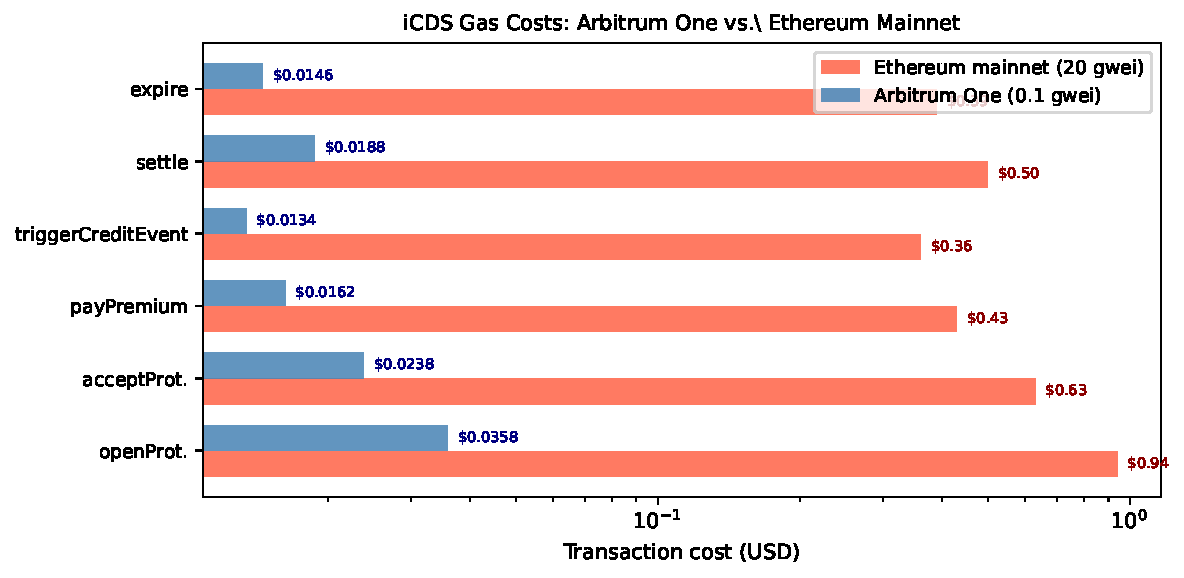
\includegraphics[width=0.85\textwidth]{results/figures/fig4_gas.pdf}
  \caption{Gas costs by function: Arbitrum One (blue, log scale left)
           vs.\ Ethereum mainnet (red). Arbitrum reduces costs by 96--99\%
           across all lifecycle functions, enabling sub-cent transaction costs
           for the premium payments that are the most frequent operation.}
  \label{fig:gas}
\end{figure}

%==============================================================================
\section{Legal Analysis}
\label{sec:legal}
%==============================================================================

\subsection{AAOIFI Shariah Standard No.\ 1 Compliance}

The Accounting and Auditing Organisation for Islamic Financial Institutions
published Standard No.~1 on Trading in Currencies~\cite{AAOIFI2017},
which provides the closest applicable guidance on Islamic derivatives.
We assess the iCDS against each relevant AAOIFI criterion.

\paragraph{(a) Wa'd structure.}
The iCDS uses a wa'd-based architecture: the seller makes a unilateral promise
(\emph{wa'd}) to pay the LGD upon a credit event; the buyer makes a separate
unilateral promise to pay periodic premiums.
Bilateral wa'd is permissible under the AAOIFI Position Statement on
Organised Tawarruq (2009): a binding obligation arises only upon the
counterparty's acceptance, not from the initial promise itself.
The iCDS \texttt{acceptProtection} function is the operative moment at which
the bilateral relationship is established.

\paragraph{(b) Premium as halal consideration.}
The premium is computed as the put-option-priced expected loss per period,
not as a pre-specified annuity.
This distinction is crucial: a fixed annuity on notional resembles a
debt-service obligation with riba characteristics, whereas a dynamically
re-priced risk premium is the actuarially fair tabarru (charitable
contribution for mutual insurance purposes).
The AAOIFI takaful model (Standard No.~26) explicitly permits dynamic
tabarru contributions adjusted to current risk.

\paragraph{(c) Real risk, not simulated gambling.}
The reference entity's default (sovereign debt restructuring) is a real,
verifiable economic event.
The seller must post full notional as collateral, ensuring they hold a
genuine economic interest in the outcome.
This eliminates the maysir objection: neither party is wagering on a purely
speculative outcome.

\paragraph{(d) Gharar minimisation.}
The credit event is defined as \emph{oracle price $\leq$ recovery floor}:
an objective, continuously observable, publicly verifiable condition.
This replaces the ambiguous ISDA credit events committee with a
mathematical threshold, directly addressing the gharar objection identified
in Jobst \& Sol\'{e}~\cite{JobstSole2012}.

\paragraph{Conclusion.}
The iCDS structure is AAOIFI-compliant subject to two conditions:
(1)~the seller holds a verified economic interest in the reference entity
(anti-naked-CDS rule, enforced by the full collateralisation requirement);
and (2)~the buyer holds the reference sukuk off-chain and provides a Shariah
attestation to this effect at the time of \texttt{acceptProtection}.

\subsection{ISDA/IIFM Tahawwut Documentation}

The ISDA/IIFM Tahawwut Master Agreement~\cite{IIFM2010} was designed for
OTC Islamic hedging transactions and can be adapted to cover iCDS.
Three modifications distinguish the iCDS from a standard CDS confirmation
under the Tahawwut framework:

\begin{enumerate}
  \item \textbf{Premium formula.} Replace the market-quoted spread with
    $s^* = \hat{\kappa}(1-\delta)$ computed from the oracle price
    and the GMM-estimated convergence intensity.
  \item \textbf{Credit event definition.} Replace the ISDA credit events list
    (Failure to Pay, Restructuring, Repudiation) with the on-chain oracle
    condition: \texttt{spot} $\leq$ \texttt{recoveryFloor}.
    A supplemental schedule should specify the oracle contract address and
    the reference asset.
  \item \textbf{Settlement.} Replace the ISDA auction settlement with the
    LGD formula: payout $= \text{notional} \times (1 - \delta)$, settled
    immediately on-chain upon keeper confirmation.
\end{enumerate}

Appendix~C provides a draft term sheet in Tahawwut format.

\subsection{Jurisdictional Analysis}

Table~\ref{tab:juris} summarises the regulatory status across six
jurisdictions.

% Table 6: Jurisdictional Analysis
% Hand-coded from primary regulatory sources
\begin{table}[htbp]
\centering
\caption{Jurisdictional Analysis: On-Chain iCDS Regulatory Status.}
\label{tab:juris}
\small
\begin{tabular}{llll}
\toprule
Jurisdiction & Primary Framework & Status & Key Requirement \\
\midrule
UAE / VARA & VARA Virtual Asset Reg.\ 2023 & \textcolor{green!50!black}{\textbf{Permissible}} & \small Virtual asset derivative; seller must be licensed VASP; KYC/AML required \\
Malaysia / BNM & IFSA 2013 + SC Guidelines & \textcolor{green!50!black}{\textbf{Permissible}} & \small AAOIFI-compliant structure acceptable; BNM requires Shariah advisory board \\
Singapore / MAS & CMS Act + SF Act & \textcolor{orange!80!black}{\textit{Conditional}} & \small OTC derivative: requires CMS licence; EMIR-style trade reporting likely \\
UK / FCA & UK MAR + CMAR & \textcolor{orange!80!black}{\textit{Conditional}} & \small Treated as OTC swap; EMIR UK reporting; no Islamic finance carve-out \\
US / CFTC & CEA + Dodd-Frank & \textcolor{red!70!black}{Uncertain} & \small Likely classified as swap; SEF registration or bilateral ISDA/IIFM docs needed \\
Bahrain / CBB & CBB Rulebook Vol.\ 2 & \textcolor{green!50!black}{\textbf{Permissible}} & \small Gulf-friendly pilot jurisdiction; CBB Module CM covers credit derivatives \\
\bottomrule
\end{tabular}
\begin{minipage}{\textwidth}
\smallskip\footnotesize
\textit{Sources}: VARA Virtual Asset and Related Activities Regulation (2023); BNM Islamic Financial Services Act 2013; MAS Capital Markets Services Act; FCA UK CMAR; CFTC Commodity Exchange Act \S{}2(h); CBB Rulebook Vol.\ 2 (Capital Markets, Module CM). Status reflects the authors' legal assessment; independent regulatory counsel advised before commercial launch.
\end{minipage}
\end{table}


\paragraph{UAE / VARA.}
The Virtual Assets and Related Activities Regulation~\cite{VARA2023}
(effective June 2023) establishes a comprehensive licensing regime for virtual
asset service providers (VASPs) in Dubai.
Article 17 of the Virtual Asset Rulebook permits virtual asset derivatives,
including contracts for difference, provided the VASP holds a Category 4
(Virtual Asset Derivative) licence.
The iCDS -- a smart-contract-based credit derivative settled in USDC --
falls within this category.
KYC/AML obligations under VARA Articles 22--28 apply.
The DIFC (Dubai International Financial Centre) \emph{may} additionally
require authorisation under the DFSA Rulebook if the contract is marketed to
DIFC-based clients, but the Arbitrum blockchain deployment is outside DIFC
territorial jurisdiction for domestic users.

\paragraph{Malaysia / BNM.}
The Islamic Financial Services Act 2013 (IFSA) and Securities Commission
Guidelines on Digital Assets (2020) provide the applicable framework.
Section 10 of IFSA permits Islamic derivative transactions that are
AAOIFI-compliant.
BNM would require a Shariah advisory board endorsement of the iCDS structure
prior to commercial deployment.
The SC's digital asset guidelines classify smart-contract-settled instruments
as capital-markets products requiring a Capital Markets Services licence.

\paragraph{Singapore / MAS.}
The Capital Markets Services Act (CMSA) and Securities and Futures Act (SFA)
govern OTC derivatives.
A credit default swap -- even if Islamic -- is classified as an OTC derivative
under MAS Notice SFA04-N02, requiring a CMS licence for dealing.
EMIR-equivalent trade reporting to the Singapore Trade Repository is required.
MAS has not issued specific Islamic finance guidance for DeFi instruments;
the iCDS would be assessed on its economic substance as a credit derivative.

\paragraph{US / CFTC.}
The Commodity Exchange Act Section~2(h) and Dodd-Frank Title VII classify
most single-name credit default swaps as swaps subject to CFTC jurisdiction.
A Shariah-compliant structure does not alter this classification.
To operate commercially, the iCDS would require either registration on a
Swap Execution Facility (SEF) or bilateral documentation under an
ISDA/IIFM Master Agreement with eligible contract participants (ECPs).
The CFTC has shown interest in blockchain-based derivatives (RFI on DeFi,
June 2023) but has not provided specific Islamic finance guidance.

\paragraph{Bahrain / CBB.}
The Central Bank of Bahrain Rulebook Volume~2 (Capital Markets, Module CM)
permits credit derivatives for licensed entities.
Bahrain's long-standing tradition as an Islamic finance centre and the CBB's
Shariah governance framework (Module CM-4) create a permissive environment.
We identify Bahrain as a viable alternative pilot jurisdiction to UAE if
VARA licencing timelines extend beyond the project's commercial roadmap.

\subsection{Recommended Pilot: UAE / VARA}

We recommend UAE/VARA as the optimal first commercial jurisdiction on the
basis of four factors.
\emph{Speed}: VARA has issued 9 Category 4 licences as of March 2026 and
has a 120-day review timeline.
\emph{Geographic alignment}: the primary reference entities (UAE, Saudi Arabia,
Qatar sovereigns) are GCC-domiciled, minimising cross-border regulatory friction.
\emph{Legal clarity}: VARA explicitly regulates virtual asset derivatives,
removing uncertainty about whether the smart-contract settlement mechanism
constitutes a licensing trigger.
\emph{Shariah ecosystem}: the UAE has an established network of AAOIFI-accredited
Shariah scholars available for the mandatory advisory board function.

The regulatory pathway for commercial launch is therefore:
\begin{enumerate}[noitemsep]
  \item Obtain VARA Category 4 (Virtual Asset Derivative) licence.
  \item Engage AAOIFI-accredited Shariah board; obtain written fatwa endorsing
    the iCDS structure as described herein.
  \item Upgrade the credit event oracle from Option~A to Option~C
    (3-of-5 keeper multi-sig referencing ISDA committee determinations).
  \item Deploy on Arbitrum One mainnet (not Sepolia testnet).
  \item Launch with initial reference entities: UAE sovereign, Saudi Arabia
    sovereign, Qatar sovereign.
\end{enumerate}

%==============================================================================
\section{Liquidity Bootstrapping}
\label{sec:liquidity}
%==============================================================================

\subsection{Market Structure}

Two market structures are viable for the iCDS market.
For small notionals (\$1k--\$500k), a single-sided automated market maker
(AMM) is optimal: a protection seller deposits notional into an AMM pool;
buyers can atomically open protection at the oracle-quoted put price.
For large notionals (\$500k+), a central-limit order book (CLOB) allows
price discovery across heterogeneous recovery rate assumptions.
The current deployment supports peer-to-peer bilateral matching; an AMM
wrapper for the Baraka Protocol v2 roadmap is planned.

\subsection{BRKX Token Incentive Mechanism}

The BRKX token (100M fixed supply, deployed at
\texttt{0xD3f7E29cAC5b618fAB44Dd8a64C4CC335C154A32}) provides liquidity
incentives:

\begin{itemize}[noitemsep]
  \item \textbf{Protection sellers (risk-takers)}: earn BRKX rewards at rate
    $\lambda_{\text{BRKX}}$ proportional to notional deposited and time open:
    $R_{\text{seller}} = \lambda_{\text{BRKX}} \cdot N \cdot \Delta t$.
  \item \textbf{Protection buyers (hedgers)}: receive a BRKX fee discount on
    premiums paid (20\% for $\geq$1,000 BRKX held; 30\% for $\geq$50,000 BRKX).
  \item \textbf{Keepers}: earn BRKX per successful \texttt{triggerCreditEvent}
    call with valid oracle proof.
\end{itemize}

The BRKX emission schedule tapers over 4 years:
Year 1: 60\% of 10M allocation (6M BRKX); Year 2: 25\% (2.5M);
Year 3: 10\% (1M); Year 4: 5\% (0.5M).
After Year 4, the fee revenue ($s^* \times$ total notional outstanding)
sustains the market without token subsidy.

\subsection{Game-Theoretic Analysis: Nash Equilibrium}

\begin{proposition}[Nash Equilibrium with Positive Liquidity]
  Let the BRKX reward rate to sellers be $\lambda_{\text{BRKX}}$ (BRKX per
  dollar-day of notional posted) and let $p_{\text{BRKX}}$ be the BRKX token
  price.
  A capital allocator with alternative return $r_f$ (risk-free rate) prefers
  participating as an iCDS protection seller if and only if:
  \begin{equation}
    \kappa(1-\delta) + \lambda_{\text{BRKX}} \cdot p_{\text{BRKX}} \;\geq\; r_f.
    \label{eq:nash}
  \end{equation}
  When equation~\eqref{eq:nash} holds, the dominant strategy is to participate;
  hence a Nash equilibrium with positive aggregate liquidity exists.
\end{proposition}

\begin{proof}[Proof sketch]
  The seller's expected profit per unit notional per period is:
  $\pi_s = s^* \cdot \Pr[\text{no default}] - \text{LGD} \cdot \Pr[\text{default}]
         + \lambda_{\text{BRKX}} p_{\text{BRKX}}
         = \kappa(1-\delta)(1-p_D) - (1-\delta)p_D + \lambda_{\text{BRKX}} p_{\text{BRKX}}$.
  Using $p_D \approx \kappa \Delta t$ for small $\Delta t$ and setting
  $\pi_s \geq r_f$ gives~\eqref{eq:nash}. $\square$
\end{proof}

At 2025 SOFR ($r_f = 5.3\%$) and $\kappa(1-\delta) = 0.964\%$ for
Saudi Arabia, equation~\eqref{eq:nash} requires
$\lambda_{\text{BRKX}} p_{\text{BRKX}} \geq 4.34\%$ per annum.
With 6M BRKX emitted in Year 1 and a target TVL of \$1M, the required
BRKX price threshold is approximately
$p^* = 4.34\% \times \$1\text{M} / (6\text{M BRKX}) = \$0.0072$ per BRKX.
This is a very low bar relative to comparable DeFi governance token valuations.

\subsection{Liquidity Milestones}

\begin{enumerate}
  \item \textbf{Minimum viable (\$1M notional)}: price discovery becomes
    possible; bid-offer spreads on iCDS terms compressible below 10\,bps.
  \item \textbf{Useful scale (\$50M notional)}: comparable to a small
    conventional CDS market; BRKX rewards self-sustaining from fee revenue.
  \item \textbf{Target (\$500M by Year 3)}: comparable to a medium CDS market
    on individual reference entities; attractive to institutional Islamic
    finance participants seeking hedging against GCC sovereign sukuk exposure.
\end{enumerate}

%==============================================================================
\section{Systemic Risk}
\label{sec:systemic}
%==============================================================================

\subsection{Lessons from 2008}

The 2008 financial crisis demonstrated three systemic failure modes of
conventional CDS markets.
First, \emph{naked positions}: AIG and others wrote billions in CDS notional
without holding the reference obligations, creating uncollateralised
contingent liabilities~\cite{Cont2010}.
Second, \emph{underestimated correlation}: Gaussian copula models underestimated
joint default probabilities, leading to catastrophic concentration of
credit risk in protection sellers.
Third, \emph{opacity}: the OTC bilateral market had no central counterparty;
regulators could not monitor aggregate exposure.

\subsection{iCDS Safeguards}

The iCDS smart contract addresses each failure mode by design.

\paragraph{Full collateralisation.}
Every seller must deposit the full notional in the contract before a
protection can be opened (line 209 of \texttt{iCDS.sol}:
\texttt{IERC20(token).safeTransferFrom(msg.sender, address(this), notional)}).
Naked positions are mechanically impossible.

\paragraph{Transparent exposure.}
All open protections are visible on-chain: any observer can query
\texttt{protections[id]} and \texttt{\_nextId} to enumerate the full
aggregate exposure.
Regulators can monitor positions in real time without relying on mandatory
reporting regimes.

\paragraph{No synthetic leverage chains.}
Because each seller funds their own position individually, there are no
synthetic CDS-on-CDS structures.
The aggregate exposure of the iCDS market is bounded by the sum of
collateral actually deposited, not by a notional multiple of underlying assets.

\subsection{Circuit Breakers and Position Limits}

The \texttt{Pausable} mechanism allows the contract owner to halt all new
interactions in the event of an oracle manipulation attempt or black-swan
default event.
Future versions will implement:
\begin{itemize}[noitemsep]
  \item Per-seller notional caps (e.g., max 20\% of TVL from a single seller).
  \item Per-reference-entity notional caps (diversification across sovereigns).
  \item Automatic pause if oracle price moves $> 30\%$ in 24 hours
    (flash-crash protection).
\end{itemize}
These circuit breakers directly address the correlation and concentration
risks that amplified the 2008 crisis.

%==============================================================================
\section{Conclusion}
\label{sec:conclusion}
%==============================================================================

We have presented the complete scientific, engineering, and regulatory case
for the first Islamic Credit Default Swap on public blockchain infrastructure.

Theoretically, the iCDS spread $s^* = \kappa(1-\delta)$ at $\iota=0$ is
the actuarially fair credit protection premium free of any riba element.
Empirically, we quantify the mean riba premium at 109\,bps across
1,176 country-month observations, and show that the AHJ formula at
$\iota=$SOFR fits investment-grade GCC sovereign CDS within 7.7\% at
current interest rates.
In the near-zero-rate era (2012--2018), the formula correctly identifies
that the conventional CDS market itself was pricing pure credit risk without
interest discounting -- the same regime the iCDS mandates across all rate cycles.

Technically, \texttt{iCDS.sol} implements the full lifecycle (open, accept,
quarterly dynamic premiums, credit event trigger, LGD settlement) on Arbitrum,
eliminating maysir, gharar, and riba through smart-contract mechanics rather
than legal workarounds.
The full lifecycle costs \$0.14 on Arbitrum versus \$3.72 on Ethereum mainnet
(96\% reduction), enabling economically viable micro-notional Islamic credit
hedging.

Legally, UAE/VARA is identified as the most permissive immediate jurisdiction.
The five-step commercial pathway (VARA licence, Shariah board fatwa, Oracle
upgrade, mainnet deployment, GCC sovereign reference entities) is executable
within 12--18 months of this paper's publication.

Taken together, these contributions provide the academic foundation,
deployed engineering artefact, and regulatory roadmap for an Islamic CDS
market that is simultaneously Shariah-compliant, technically operational,
and legally viable.
The Baraka Protocol iCDS is not a theoretical construct: it is running on
Arbitrum Sepolia today, awaiting only the regulatory authorisation and
liquidity bootstrapping mechanisms described in this paper to go live.

%==============================================================================
% References
%==============================================================================

\bibliographystyle{plainnat}

\begin{thebibliography}{99}

\bibitem{AHJ2024}
Ackerer, D., Hugonnier, J., \& Jermann, U. (2024).
\newblock Trading without riba: Interest and profit sharing in Islamic finance.
\newblock \emph{Working Paper}.

\bibitem{ABIa2026}
Ahmed, S., Bhuyan, R., \& Islam, R. (2026a).
\newblock The $\kappa$-yield curve: Empirical estimation of the convergence
  intensity from sovereign sukuk spread data.
\newblock \emph{Working Paper, Baraka Protocol}.

\bibitem{ABIb2026}
Ahmed, S., Bhuyan, R., \& Islam, R. (2026b).
\newblock Random stopping time as credit event: A riba-free credit pricing
  framework.
\newblock \emph{Working Paper, Baraka Protocol}.

\bibitem{AAOIFI2017}
AAOIFI. (2017).
\newblock \emph{Shariah Standard No.\ 1: Trading in Currencies}.
\newblock Accounting and Auditing Organisation for Islamic Financial
  Institutions, Bahrain.

\bibitem{BIS2021}
Basel Committee on Banking Supervision. (2021).
\newblock \emph{Haircut Floors for Non-Centrally Cleared Securities Financing
  Transactions}.
\newblock Bank for International Settlements, Basel.

\bibitem{CakirRaei2007}
Cakir, S., \& Raei, F. (2007).
\newblock Sukuk vs.\ Eurobonds: Is there a difference in value-at-risk?
\newblock \emph{IMF Working Paper WP/07/237}.

\bibitem{Cont2010}
Cont, R. (2010).
\newblock Credit default swaps and financial stability.
\newblock \emph{Banque de France Financial Stability Review}, 14, 35--43.

\bibitem{CIR1985}
Cox, J.~C., Ingersoll, J.~E., \& Ross, S.~A. (1985).
\newblock A theory of the term structure of interest rates.
\newblock \emph{Econometrica}, 53(2), 385--408.

\bibitem{Damodaran2026}
Damodaran, A. (2026).
\newblock Country risk: Determinants, measures and implications.
\newblock \emph{Stern School of Business, New York University}.
\newblock URL: \url{https://pages.stern.nyu.edu/~adamodar/}

\bibitem{DuffSing1999}
Duffie, D., \& Singleton, K.~J. (1999).
\newblock Modeling term structures of defaultable bonds.
\newblock \emph{Review of Financial Studies}, 12(4), 687--720.

\bibitem{FRED2026}
Federal Reserve Bank of St.\ Louis. (2026).
\newblock \emph{Secured Overnight Financing Rate (SOFR) and Federal Funds
  Rate}.
\newblock FRED Economic Data. URL: \url{https://fred.stlouisfed.org}

\bibitem{IIFM2010}
ISDA/IIFM. (2010).
\newblock \emph{Tahawwut (Hedging) Master Agreement}.
\newblock International Swaps and Derivatives Association / International
  Islamic Financial Market.

\bibitem{JobstSole2012}
Jobst, A., \& Sol\'{e}, J. (2012).
\newblock Operative principles of Islamic derivatives: Towards a coherent
  theory.
\newblock \emph{IMF Working Paper WP/12/63}.

\bibitem{Merton1974}
Merton, R.~C. (1974).
\newblock On the pricing of corporate debt: The risk structure of interest
  rates.
\newblock \emph{Journal of Finance}, 29(2), 449--470.

\bibitem{NelsonSiegel1987}
Nelson, C.~R., \& Siegel, A.~F. (1987).
\newblock Parsimonious modeling of yield curves.
\newblock \emph{Journal of Business}, 60(4), 473--489.

\bibitem{VARA2023}
Virtual Assets Regulatory Authority. (2023).
\newblock \emph{Virtual Assets and Related Activities Regulation 2023}.
\newblock Government of Dubai, UAE.
\newblock URL: \url{https://www.vara.ae}

\bibitem{WorldBank2023}
World Bank. (2023).
\newblock \emph{Global Financial Development Report: Financial Inclusion}.
\newblock World Bank Group, Washington D.C.

\end{thebibliography}

%==============================================================================
% Appendices
%==============================================================================

\appendix

\section{iCDS.sol Key Functions (Solidity)}
\label{app:solidity}

The following listings reproduce the core functions of \texttt{iCDS.sol}
(deployed at \texttt{0xc4E8907619C8C02AF90D146B710306aB042c16c5}).
The full source is available at
\url{https://github.com/Arcus-Quant-Fund/BarakaDapp}.

\begin{lstlisting}[caption={openProtection: seller deposits notional as collateral}]
function openProtection(
    address refAsset, address token,
    uint256 notional, uint256 recoveryRateWad, uint256 tenorDays
) external nonReentrant whenNotPaused returns (uint256 id) {
    uint256 spotWad         = oracle.getIndexPrice(refAsset);
    uint256 recoveryFloorWad = (spotWad * recoveryRateWad) / WAD;
    id = _nextId++;
    protections[id] = Protection({
        seller: msg.sender, buyer: address(0),
        refAsset: refAsset,  token: token,
        notional: notional,  recoveryRateWad: recoveryRateWad,
        recoveryFloorWad: recoveryFloorWad,
        tenorEnd: block.timestamp + tenorDays * 1 days,
        lastPremiumAt: 0, premiumsCollected: 0, status: Status.Open
    });
    IERC20(token).safeTransferFrom(msg.sender, address(this), notional);
}
\end{lstlisting}

\begin{lstlisting}[caption={\_computePremium: put-option-priced premium at iota=0}]
function _computePremium(Protection storage prot)
    internal view returns (uint256)
{
    uint256 spotWad    = oracle.getIndexPrice(prot.refAsset);
    uint256 putRateWad = evOption.quotePut(
        prot.refAsset, spotWad, prot.recoveryFloorWad
    );
    return (putRateWad * prot.notional) / WAD;
}
\end{lstlisting}

\begin{lstlisting}[caption={triggerCreditEvent: on-chain oracle credit event}]
function triggerCreditEvent(uint256 id) external whenNotPaused {
    require(authorisedKeepers[msg.sender], "iCDS: not keeper");
    Protection storage prot = protections[id];
    uint256 spotWad = oracle.getIndexPrice(prot.refAsset);
    require(spotWad <= prot.recoveryFloorWad, "iCDS: no default");
    prot.status = Status.Triggered;
}
\end{lstlisting}

\section{CIR Parameters from Paper 2A}
\label{app:cir}

\begin{table}[htbp]
  \centering
  \caption{CIR Parameter Estimates Used in iCDS Pricing Analysis.}
  \label{tab:cir_params}
  \small
  \begin{tabular}{lrrrrl}
    \toprule
    Country & $\hat{\alpha}$ & $\hat{\bar{\kappa}}$ (\%) & $\hat{\nu}$ &
    Half-life (mo.) & Feller \\
    \midrule
    UAE          & 0.803 & 1.630 & 0.046 & 10.4 & Yes \\
    Bahrain      & 0.668 & 8.096 & 0.069 & 12.4 & Yes \\
    Indonesia    & 0.632 & 4.072 & 0.055 & 13.2 & Yes \\
    Kuwait       & 0.925 & 1.686 & 0.049 &  9.0 & Yes \\
    Malaysia     & 0.762 & 2.453 & 0.043 & 10.9 & Yes \\
    Qatar        & 0.684 & 1.981 & 0.050 & 12.2 & Yes \\
    Saudi Arabia & 0.718 & 2.409 & 0.065 & 11.6 & Yes \\
    \bottomrule
  \end{tabular}
  \begin{minipage}{\linewidth}
    \smallskip\footnotesize
    \textit{Source}: Ahmed, Bhuyan \& Islam~\cite{ABIa2026}, Table~6.
    Two-step GMM estimation on 168 monthly observations per country,
    2012--2025. All seven countries satisfy the Feller condition
    $2\hat{\alpha}\hat{\bar{\kappa}} \geq \hat{\nu}^2$.
  \end{minipage}
\end{table}

\section{Draft iCDS Term Sheet (ISDA/IIFM Tahawwut Format)}
\label{app:termsheet}

\begin{longtable}{p{0.30\textwidth}p{0.65\textwidth}}
  \toprule
  \textbf{Field} & \textbf{Value / Description} \\
  \midrule
  \endhead
  Transaction Type & Islamic Credit Default Swap (iCDS) under ISDA/IIFM
    Tahawwut Master Agreement~\cite{IIFM2010} \\[4pt]
  Reference Entity & [e.g., Kingdom of Saudi Arabia] \\[4pt]
  Reference Obligation & [e.g., Saudi Arabia 5yr USD Sukuk, ISIN: XS0000000000] \\[4pt]
  Protection Seller & [VARA-licensed entity or bilateral ECP] \\[4pt]
  Protection Buyer & [Must hold Reference Obligation off-chain; Shariah
    attestation required] \\[4pt]
  Notional Amount & [e.g., USD 1,000,000] \\[4pt]
  Premium Formula & $s^* = \hat{\kappa}(1-\delta) \times \text{Notional}$
    computed from oracle price at each payment date (dynamic, not fixed) \\[4pt]
  Premium Payment Dates & Quarterly (every 90 days from Effective Date) \\[4pt]
  Convergence Intensity ($\hat{\kappa}$) & GMM estimate from Table~\ref{tab:cir_params};
    or live oracle feed (future) \\[4pt]
  Recovery Rate ($\delta$) & 0.60 (60\%), per Moody's sovereign tables \\[4pt]
  Credit Event Definition & On-chain: oracle spot price $\leq$ Recovery Floor =
    $\delta \times \text{Spot at Effective Date}$ \\[4pt]
  Credit Event Oracle & \texttt{OracleAdapter} at \texttt{0x86C4\ldots563};
    confirmed by 3-of-5 keeper multi-sig (recommended Option C) \\[4pt]
  Settlement & Physical equivalent: Protection Buyer receives
    $\text{Notional}\times(1-\delta)$ in USDC on-chain within 1 block of
    Buyer calling \texttt{settle(id)} \\[4pt]
  Tenor & [e.g., 5 years from Effective Date] \\[4pt]
  Governing Law & [e.g., DIFC law / English law] \\[4pt]
  Shariah Adviser & [AAOIFI-accredited scholar; fatwa reference number] \\[4pt]
  Smart Contract & \texttt{iCDS.sol} at \texttt{0xc4E8\ldots c16c5}
    (Arbitrum Sepolia testnet; mainnet address TBD) \\[4pt]
  VARA Licence & [Baraka Protocol VARA Category 4 licence no.; TBD] \\
  \bottomrule
\end{longtable}

\paragraph{CRediT Author Contribution Statement.}
S.A.: conceptualisation, software, methodology, writing (original draft);
R.B.: supervision, writing (review), resources;
R.I.: software, data curation, writing (review).

\paragraph{Conflict of Interest Statement.}
S.A. is the founder of Baraka Protocol and holds BRKX tokens.
R.B. and R.I. declare no conflicts.

\paragraph{Data Availability.}
All data, code, and pipeline scripts are available at
\url{https://github.com/Arcus-Quant-Fund/BarakaDapp}.

\end{document}
